% this file is called up by thesis.tex
% content in this file will be fed into the main document

%: ----------------------- name of chapter  -------------------------
\chapter{Bilaga} % top level followed by section, subsection
\label{bilaga}

%: ----------------------- paths to graphics ------------------------
\ifpdf
    \graphicspath{{10_bilaga/figures/PNG/}{10/figures/PDF/}{10/figures/}}
\else
    \graphicspath{{10_bilaga/figures/EPS/}{10/figures/}}
\fi

\graphicspath{{10_bilaga/figures/}{10/figures/}}

%: ----------------------- contents from here ------------------------


\section{GitHub-länk}

\begin{itemize}
\item http://github.com/MalmoUniversity-DA264A/SAFE24.git/
\end{itemize}


\section{Diagram}

\begin{figure}[h]
  \includegraphics[width=\linewidth, height=22cm]{diagram.png}
  \caption{Flödesdigram för systemet.}
  \label{fig:diagram}
\end{figure}

\begin{figure}[h]
  \includegraphics[width=\linewidth]{diagramSensor.png}
  \caption{Flödesdigram för metoden doWithSensorValues.}
  \label{fig:diagramSensor}
\end{figure}

\begin{figure}[h]
  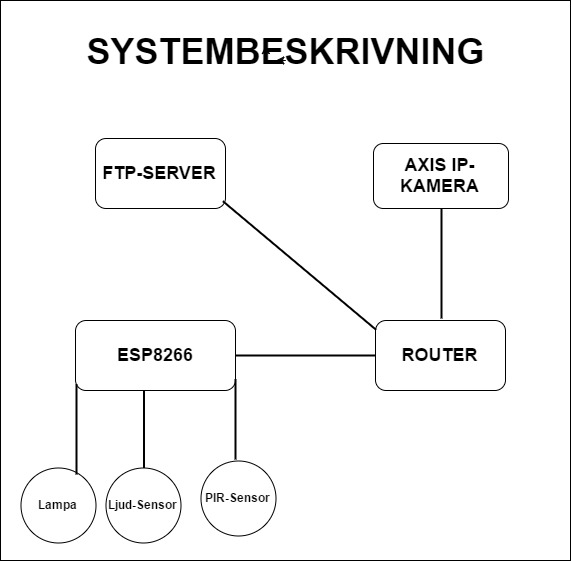
\includegraphics[width=\linewidth]{Systembeskrivning.jpg}
  \caption{Systembeskrivning}
  \label{fig:Systembeskrivning}
\end{figure}

\clearpage

\section{Testfall}

\begin{figure}[h]
  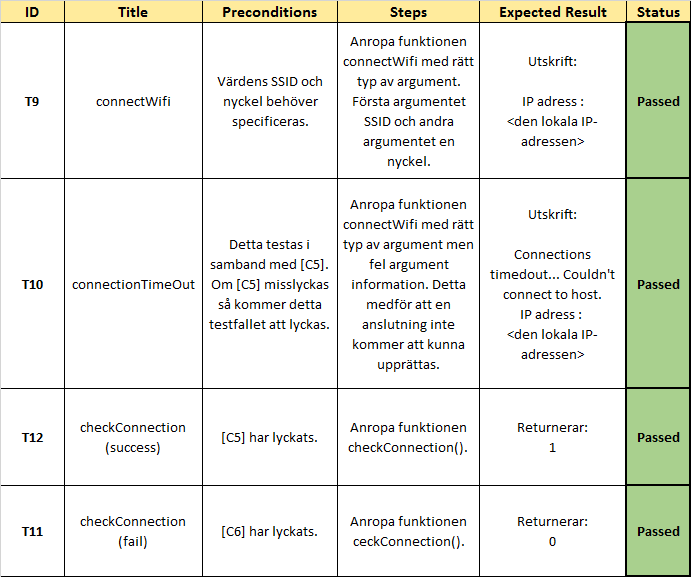
\includegraphics[width=\linewidth]{Anslutningstest.png}
  \caption{Testfall för anslutning}
  \label{fig:Anslutningstest}
\end{figure}

\begin{figure}[h]
  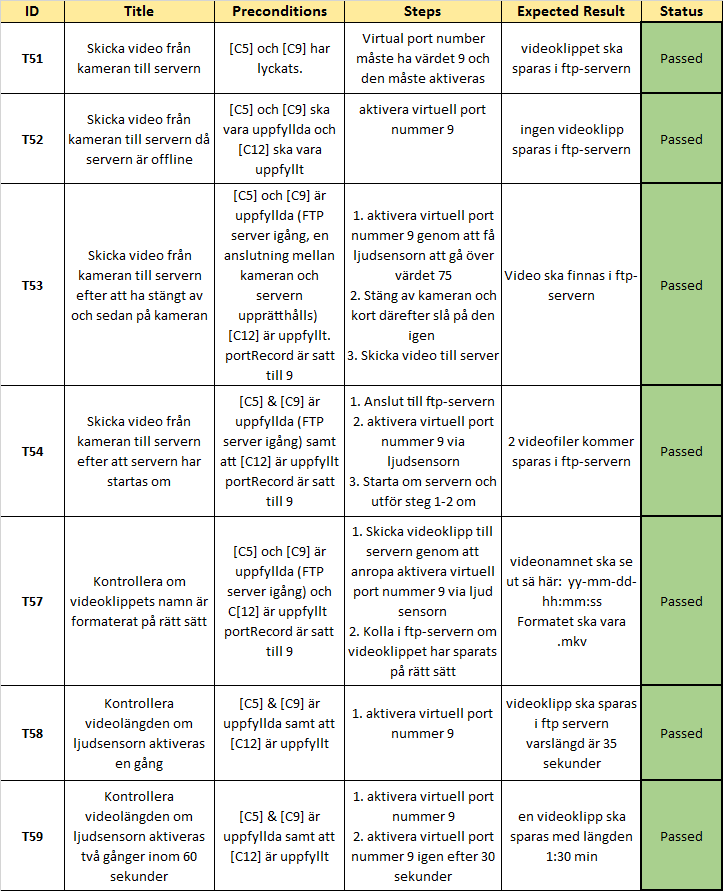
\includegraphics[width=\linewidth]{FTPTest.png}
  \caption{Testfall för FTP server}
  \label{fig:FTPTest}
\end{figure}

\begin{figure}[h]
  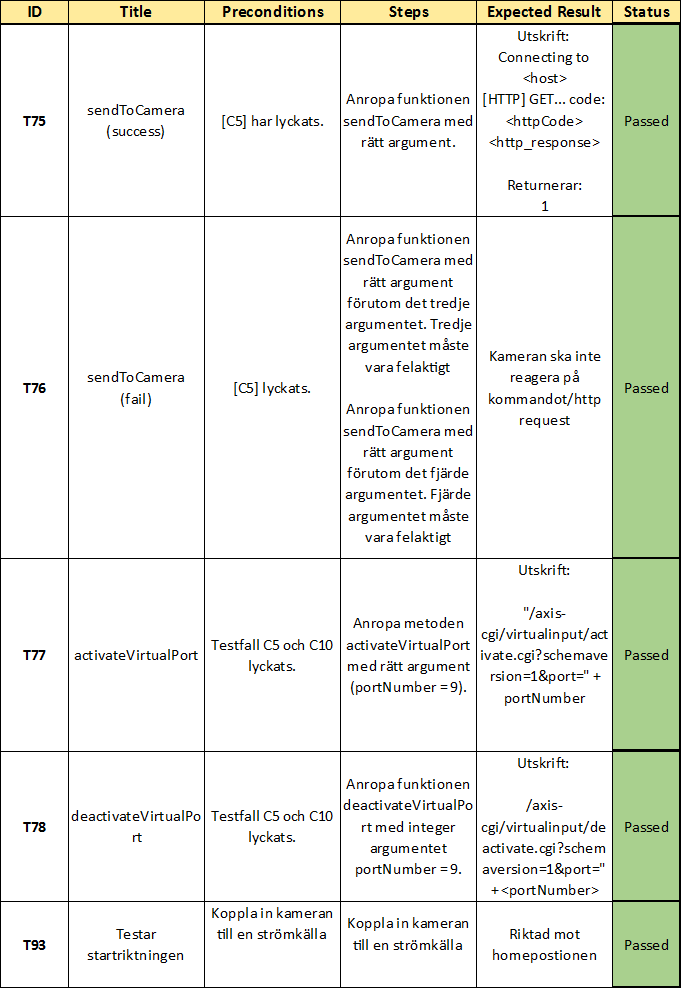
\includegraphics[width=\linewidth]{HanteraIPKameraTest1.png}
  \label{fig:HanteraIPKameraTest1}
\end{figure}

\newpage

\begin{figure}[h]
  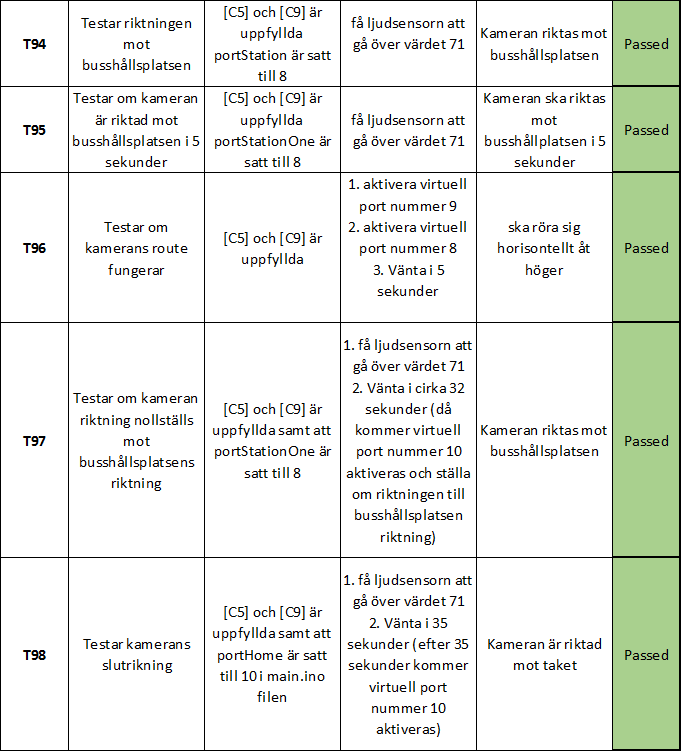
\includegraphics[width=\linewidth]{HanteraIPKameraTest2.png}
  \caption{Testfall för IP kamera}
  \label{fig:HanteraIPKameraTest2}
\end{figure}


\begin{figure}[h]
  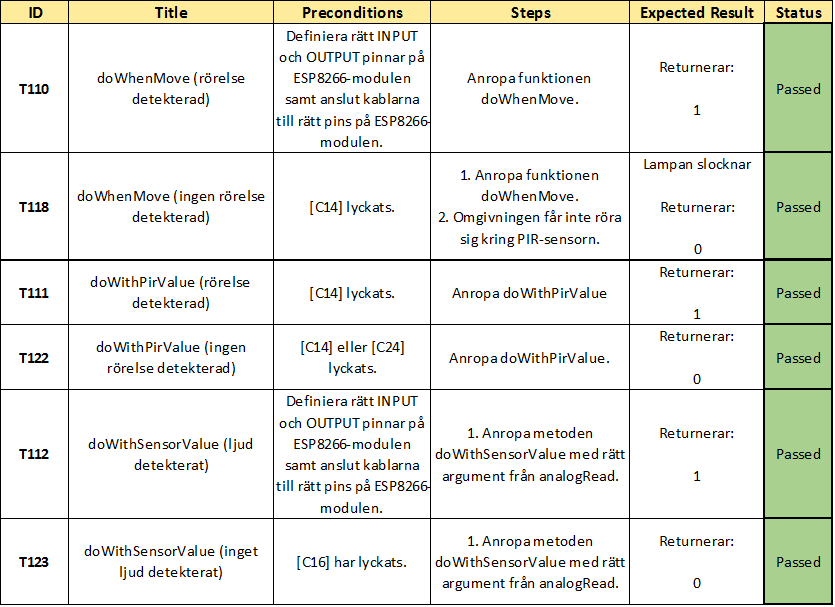
\includegraphics[width=\linewidth]{SensorTest.png}
  \caption{Testfall för sensorerna}
  \label{fig:SensorTest}
\end{figure}

\begin{figure}[h]
  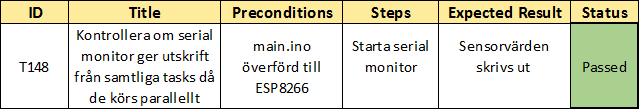
\includegraphics[width=\linewidth]{SchedulingTest.png}
  \caption{Testfall för multitasking}
  \label{fig:SchedulingTest}
\end{figure}



% ---------------------------------------------------------------------------
%: ----------------------- end of thesis sub-document ------------------------
% ---------------------------------------------------------------------------

